% Some shortcuts adapted from https://math.mit.edu/~psh/amshelp/2.3/template.tex

\documentclass[]{article}
\usepackage[utf8]{inputenc}
\usepackage{geometry}
% \usepackage{yfonts}
% \usepackage{xfrac}
% \usepackage[c]{esvect}
% \usepackage{setspace}
\usepackage{eurosym}
\usepackage{caption}
\usepackage{subcaption}
\usepackage{graphicx}
\usepackage{indentfirst}
\usepackage{amsmath,amsfonts,amsthm,amscd,upref,amstext}	
\usepackage{amssymb}
\usepackage{mathtools}
\usepackage[all,cmtip]{xy}
\input xy
\xyoption{all}
\usepackage{hyperref}
\usepackage[]{amsrefs} % amsrefs must be loaded after hyperref
\usepackage{tikz}
%\usepackage{etoolbox} % for \ifthen
\usepackage{listofitems} % for \readlist to create arrays
\usepackage[outline]{contour} % glow around text
\usepackage{xcolor}
\usetikzlibrary{arrows.meta} % for arrow size
\contourlength{1.4pt}
\tikzset{>=latex} % for LaTeX arrow head
\colorlet{myRed}{red!80!black}
\colorlet{myBlue}{blue!80!black}
\colorlet{myGreen}{green!60!black}
\colorlet{myOrange}{orange!70!red!60!black}
\colorlet{myDarkBlue}{blue!40!black}
\colorlet{myDarkGreen}{green!30!black}
\tikzstyle{node}=[thick,circle,draw=myBlue,minimum size=22,inner sep=0.5,outer sep=0.6]
\tikzstyle{node in}=[node,green!20!black,draw=myDarkGreen!30!black,fill=myGreen!25]
\tikzstyle{node hidden}=[node,blue!20!black,draw=myBlue!30!black,fill=myBlue!20]
\tikzstyle{node convol}=[node,orange!20!black,draw=myOrange!30!black,fill=myOrange!20]
\tikzstyle{node out}=[node,red!20!black,draw=myRed!30!black,fill=myRed!20]
\tikzstyle{connect}=[thick,myDarkBlue] %,line cap=round
\tikzstyle{connect arrow}=[-{Latex[length=4,width=3.5]},thick,myDarkBlue,shorten <=0.5,shorten >=1]
\tikzset{ % node styles, numbered for easy mapping with \nstyle
  node 1/.style={node in},
  node 2/.style={node hidden},
  node 3/.style={node out},
}
\def\nstyle{int(\lay<\Nnodlen?min(2,\lay):3)} % map layer number onto 1, 2, or 3
\def\svmybf#1{\rotatebox{90}{\stretchto{\{}{#1}}}
\def\svnobf#1{}
\def\rlwd{.5pt}

\newcommand{\itilde}{\tilde{\imath}}
\newcommand{\jtilde}{\tilde{\jmath}}
\newcommand{\ihat}{\hat{\imath}}
\newcommand{\jhat}{\hat{\jmath}}
\def \mat#1{\underline{\underline{#1}}}

%%%-------------------------------------------------------------------
%%%-------------------------------------------------------------------
%%% The Theorem environments:
%%%
%%%
%%% The following commands set it up so that:
%%% 
%%% All Theorems, Corollaries, Lemmas, Propositions, Definitions,
%%% Remarks, Examples, Notations, and Terminologies  will be numbered
%%% in a single sequence, and the numbering will be within each
%%% section.  Displayed equations will be numbered in the same
%%% sequence. 
%%% 
%%% 
%%% Theorems, Propositions, Lemmas, and Corollaries will have the most
%%% formal typesetting.
%%% 
%%% Definitions will have the next level of formality.
%%% 
%%% Remarks, Examples, Notations, and Terminologies will be the least
%%% formal.

\numberwithin{equation}{section}

\theoremstyle{plain} %% This is the default, anyway
\newtheorem{thm}[equation]{Theorem}
\newtheorem{cor}[equation]{Corollary}
\newtheorem{lem}[equation]{Lemma}
\newtheorem{prop}[equation]{Proposition}

\theoremstyle{definition}
\newtheorem{defn}[equation]{Definition}

\theoremstyle{remark}
\newtheorem{rem}[equation]{Remark}
\newtheorem{ex}[equation]{Example}
\newtheorem{notation}[equation]{Notation}
\newtheorem{terminology}[equation]{Terminology}
% \usepackage[titletoc]{appendix}

%%%-------------------------------------------------------------------

\title{Modelling Green Energy Conversion Networks for Generating Hydrogen Electric Vehicle Fuel}
\author{Lucas Ng\footnote{University of Cambridge, E-mail: ln373@cam.ac.uk}}
\date{\today}

%%%-------------------------------------------------------------------

\begin{document}
\maketitle
\abstract{
    \noindent Investigating the feasibility of using hydrogen as a fuel for electric vehicles
    requires a robust techno-economic comparison and feasibility analysis to determine its suitability
    as a competitor to pre-existing market alternatives. The relationships between two major abstractions
    in energy conversion networks---energy stores/resources and energy converters---were considered and explored,
    being modelled as a simple, directed, weakly-connected graph. This abstraction permits the formalisation
    of state-dependent operators that can be applied to numerically integrate the state of the network
    over time, hence permitting the utilisation of the dynamic programming methods to analyse and optimise potential systems
    subject to techno-economic constraints.
}
\newpage
\section{Introduction}

The global shift away from fossil fuels towards renewable energy sources
necessitates highly efficient and effective energy conversion networks.
Thus it is increasingly important to develop robust methods for modelling and analysing
the behaviour of such networks in order to determine their feasibility and optimise their performance.

One such network is the system for generating hydrogen as a fuel for electric vehicles (HEVs).
This simplified linear instance of such a system demonstrates the key features:
$$\overset{\text{Sun}}{\bullet} \xrightarrow[\text{PV cells}]{} \overset{\text{Battery}}{\bullet} \xrightarrow[\text{Electrolyser,\ Compressor}]{} \overset{H_{2} \text{ fuelling station}}{\bullet}$$

This graphical abstraction of the system is useful for visualising the relationships between the various components.
Moreover, it is possible to formalise the relationships between the components as a directed graph.
Notice that the Sun, Battery and $\mathrm{H_2}$ fuelling station are energy stores
if an energy resource can be considered as an energy store of pseudo-infinite capacity.
The PV cells, electrolyser and compressor are energy converters which take a single input and produce a single output.

Treating energy stores as graph vertices and energy converters as weighted graph edges
provides a general approach that can be utilised to model the behaviour of broad class of energy conversion networks.
This class can be further broadened by transforming other networks into this form,
for example by edge subdivisions or adjusting edge weightings.

The attribute of generality is important for the model to be of utility for future investigation.
One pertinent use case is a large-scale network of many HEV fuelling stations.
It is especially crucial to be able to model the behaviour under critical conditions such as component failure.
This is because the failure of a single component can have a significant impact on the performance of the entire system.

\begin{center}
    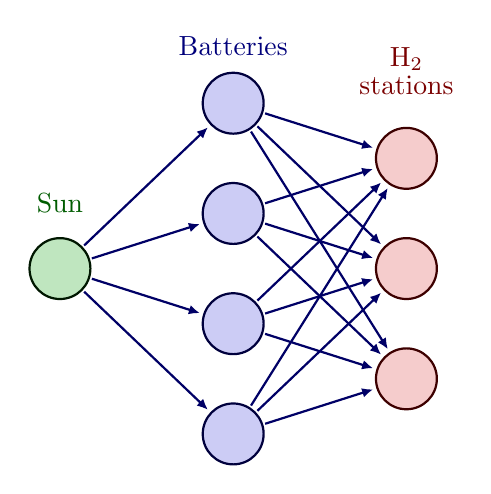
\begin{tikzpicture}[x=2.2cm,y=1.4cm]
        % Adapted from https://tikz.net/neural_networks/
        \message{^^JNeural network with arrows}
        \readlist\Nnod{1,4,3} % array of number of nodes per layer
        \message{^^J  Layer}
        \foreachitem \N \in \Nnod{ % loop over layers
            \edef\lay{\Ncnt} % alias of index of current layer
            \message{\lay,}
            \pgfmathsetmacro\prev{int(\Ncnt-1)} % number of previous layer
            \foreach \i [evaluate={\y=\N/2-\i; \x=\lay; \n=\nstyle;}] in {1,...,\N}{ % loop over nodes
                    % NODES
                    \node[node \n] (N\lay-\i) at (\x,\y){}; %{$u_\i^{(\prev)}$};
                    % CONNECTIONS
                    \ifnum\lay>1 % connect to previous layer
                        \foreach \j in {1,...,\Nnod[\prev]}{ % loop over nodes in previous layer
                                \draw[connect arrow] (N\prev-\j) -- (N\lay-\i); % connect arrows directly
                            }
                    \fi % else: nothing to connect first layer
                }
        }
        % LABELS
        \node[above=5,align=center,myGreen!60!black] at (N1-1.90) {Sun};
        \node[above=2,align=center,myBlue!60!black] at (N2-1.90) {Batteries};
        \node[above=8,align=center,myRed!60!black] at (N\Nnodlen-1.90) {$\mathrm{H_2}$\\[-0.2em]stations};

    \end{tikzpicture}
\end{center}

In the above example, the high connectivity and number of nodes per layer will likely prevent a single battery failure from entirely disabling its downstream components,
but having a mathematical way to quantify the benefit of this connectivity
is critical for determining the trade-off between economics and system performance.

The objective of this article is to develop a generalised model for analysing the behaviour of such energy conversion networks

\section{Methodology}
\subsection{Preliminaries}
% It is of utility to formalise the relationships between the various components of the network as a graph.
Consider a simple, directed graph defined as an ordered pair of vertices and edges $G = (V, E)$
where $V$ is the vertex-set and $E\subseteq\left \{(x,y):(x,y)\in V^2\ |\ x\neq y\right \}$ is the directed edge-set, with vertices labelled to represent the \emph{energy stores}
and edges labelled to represent the \emph{energy converters} of the energy system.
\begin{defn}
    The \emph{adjacency matrix} of $G$ is $\mat A\in\mathbb{R}^{V\times V}$ such that its entries satisfy
    $$\mat A_{ij} = \left [(v_i, v_j)\in E \right ]$$
    where $[\ \cdot\ ]$ is the Iverson bracket.
\end{defn}
\begin{defn}
    Similarly, the \emph{weighted adjacency matrix} of $G$ is $\mat W\in\mathbb{R}^{V\times V}$ such that its entries satisfy
    $$\mat W_{ij} = w(i, j)\mat A_{ij}$$
    where $w(i, j)$ is the weight label of the edge $(v_i, v_j)$.
\end{defn}

\begin{lem}
    $G$ is connected iff $\nexists\ (i, j)$ such that $$\left (\sum_{k = 1}^{|V|} \mat{A}^k\right )_{ij}=0$$
\end{lem}
\begin{proof}
    $\mat A$ is a linear map between vertices and their neighbours so
    $(\mat{A}^k)_{ij}$ is the number of $k$-walks from $v_i$ to $v_j$.
    Hence the total number of walks from $v_i$ to $v_j$ in $K$ steps or less is given by
    $\left (\sum_{k = 1}^{K}\mat{A}^k\right )_{ij}$.
    Now, if a walk between $v_i$ and $v_j$ exists,
    the shortest such walk must be in a number of steps less than or equal to the cardinality of $V$,
    that is, $G$ is connected iff the number of walks in $|V|$ steps or less between every pair of vertices is non-zero.
\end{proof}
\begin{lem}
    $G$ is weakly connected iff $\nexists\ (i, j)$ such that $$\left (\sum_{k = 1}^{|V|} \left (\mat{A}+\mat{A}^\top\right )^k\right )_{ij}=0$$
\end{lem}
\begin{proof}
    A directed graph is weakly connected if its underlying undirected graph is connected.
    Since $A^\top$ is the adjacency matrix for the graph with the same vertices as $G$ and reversed edges compared to $G$,
    the adjacency matrix $\mat A^\prime$ for the underlying undirected graph of $G$ has the same zero-entries as $\mat A+\mat A^\top$, that is to say
    $$\forall i, j: [\mat A^\prime_{ij} = 0]\Leftrightarrow [(\mat A+\mat A^\top)_{ij} = 0]  $$
    Hence the result follows from the previous lemma.
\end{proof}
This latter lemma serves as a useful tool for asserting the weak connectivity of a graph in the model
since disconnected graphs will be considered to be separate systems.

\subsection{Ideal Behaviour}
To develop the model, first begin by examining the ideal case without constraints or energy losses.
Consider a single vertex $v_i\in V$ representing an energy storage unit (e.g., a $\mathrm{H_2}$ fuelling station) labelled with its stored energy $u_i=u_i(t)$:
$$\xrightarrow[\text{Net power in}]{}\overset{u_i(t)}{\bullet} \xrightarrow[\text{Net power out}]{}$$

In the ideal case the flow of energy through the vertex from and to its neighbours is unrestricted and immediate. During a time interval $\varDelta t$
$$\varDelta u_i(t)=u_i(t+\varDelta t)-u_i(t)=-\overbrace{\sum_{j=1}^{N}\mat W_{ij}u_i(t)}^{\text{energy out}}+\underbrace{\sum_{j=1}^{N}\mat W_{ji}u_j(t)}_{\text{energy in}}$$

Future references to this result will omit the explicit declarations of $\underline u$ being a function of time for brevity,
however these terms should still be understood to be time-dependent.
It is also useful to sanity-check that this result is consistent with the First Law of Thermodynamics:

\begin{lem}
    $\forall\ \mat W,\underline{u}:\sum_{i=1}^{N}\varDelta u_i=0$
\end{lem}
\begin{proof}
    $$\sum_{i=1}^{N}\varDelta u_i=\sum_{i=1}^{N}\left (-\sum_{j=1}^{N}\mat W_{ij} u_i+\sum_{j=1}^{N}\mat W_{ji}u_j\right )=\sum_{i=1}^{N}\sum_{j=1}^{N}\mat W_{ji}u_j-\sum_{j=1}^{N}\sum_{i=1}^{N}\mat W_{ij}u_i=0$$
\end{proof}

Thus this process conserves $\left\lVert {\underline u}\right\rVert$ and is diffusive.

\subsection{Non-Ideal Behaviour}
The model considers the following non-idealities:
\begin{itemize}
    \item \textbf{Maximum storage capacity} $u_{i_{max}}$ such that $0\leq u_{i}\leq u_{i_{max}}$.
    \item \textbf{Maximum energy transfer rate} $\mat P_{ij}$ such that $0\leq\mat W_{ij}u_i\leq\mat P_{ij}\varDelta t$ where $\mat P_{ij}$ is the maximum possible power transfer through the edge $(v_i,v_j)$.
    \item \textbf{Energy storage self-discharge}: loss of energy stored over time.
    \item \textbf{Power transfer inefficiency}: losses during energy conversion.
\end{itemize}

The constraints on maximum energy and power can be handled by applying bounds to some of the terms in the prior result.
$$
    \varDelta u_i = \min \left( u_{i_{\mathrm{max}}}-u_i, \begin{aligned}
         & -\sum_{j=1}^{N}\min(\mat W_{ij}u_i,\mat P_{ij}\varDelta t) \\
         & +\sum_{j=1}^{N}\min(\mat W_{ji}u_j,\mat P_{ji}\varDelta t)
    \end{aligned} \right)
$$
It is now no longer guaranteed that $\sum_{i=1}^{N}\varDelta u_i=0$ because the system is no longer closed.
\bigbreak
To handle self-discharge losses and energy conversion losses, consider an arbitrary energy conversion $p_{xy}$ with efficiency $\eta_p$.
For simplicity, assume in this example that $p_{xy}$ is the only edge out of $v_x$
and assume initially that $p_{xy}$ is ideal, that is, $\eta_p=1$.
$$\overset{v_x}{\bullet}\xrightarrow{\qquad p_{xy},\ \eta_p = 1\qquad}\overset{v_y}{\bullet}$$
If $p$ is not, in fact, ideal, then we can model this by partitioning some power off into an energy wastage sink.
Suppose it is 70\% efficient:

$$
    \xymatrix@C=3em@R=3em{
    \overset{v_x}{\bullet}\ar@{-->}[ddr]^{30\%}\ar@{->}[rr]^{p_{xy},\ \eta_p = 70\%} &&\overset{v_y}{\bullet}\ar@{} \\
    \\
    &\underset{\mathrm{energy\ sink}}{\bullet}\ar@{}
    }
$$
Additionally, suppose that $v_x$ has a self-discharge rate of 10\%/$\varDelta t$.
Then the net useful power out of $v_x$ is $\eta_p(p_{xy}-\frac{0.1}{\varDelta t}u_x)$.
To keep the graph simple, combine the two edges representing power loss into a single one.

\begin{minipage}[c]{0.3\textwidth}
    $$
        \xymatrix@C=3em@R=3em{
        \overset{v_x}{\bullet}\ar@{-->}[ddr]^{27\%}\ar@{-->}@/_2em/[ddr]_{10\%}\ar@{->}[rr]^{p_{xy},\ \eta_p = 63\%} &&\overset{v_y}{\bullet}\ar@{} \\
        \\
        &\underset{\mathrm{energy\ sink}}{\bullet}\ar@{}
        }
    $$

\end{minipage}
\hspace{0.045\textwidth}
\begin{minipage}[c]{0.1\textwidth}
    \Large$$\xrightleftharpoons{\hspace{1em}}$$
\end{minipage}
\hspace{0.05\textwidth}
\begin{minipage}[c]{0.3\textwidth}
    $$
        \xymatrix@C=3em@R=3em{
        \overset{v_x}{\bullet}\ar@{-->}[ddr]^{37\%}\ar@{->}[rr]^{p_{xy},\ \eta_p = 63\%} &&\overset{v_y}{\bullet}\ar@{} \\
        \\
        &\underset{\mathrm{energy\ sink}}{\bullet}\ar@{}
        }
    $$
\end{minipage}
\bigbreak
Now that the model has been extended to handle non-idealities, it is possible to consider the behaviour of the system over time
through numerical integration by successive summation of $\varDelta u_i$.

\section{Results}
Returning to the initial simple linear system considered
$$\overset{\text{Sun}}{\bullet} \xrightarrow[\text{PV cells}]{} \overset{\text{Battery}}{\bullet} \xrightarrow[\text{Electrolyser,\ Compressor}]{} \overset{H_{2} \text{ fuelling station}}{\bullet}$$
applying the model to this system yields some interesting results,
with data about photovoltaic performance sampled for Cyprus.
Assumptions about system component characteristics were taken to be
the same as Olympios et al. \cite{olympios2023technology}.
The modelling and optimisation was implemented in \emph{Python}.
\bigbreak
The model was applied in the context of a techno-economic optimisation problem.
The \emph{L-BFGS-B} algorithm was used to minimise the total budget required to sustain the system for a given number of HEV consumers.
The results for the optimal budget allocation between system components is given in Figure \ref{fig:min_budget}.
Note that the solution $\eta$ given is relative to the output of the PV cells.

\begin{figure}[htbp]
    \centering
    \begin{tabular}{|c||c|c|c|}
        \hline
        \# HEVs & Min. budget (\euro{}) & Solution $\eta$ & PV capacity (kW) \\
        \hline
        1       & 70.8k                 & 0.55            & 4.6              \\
        10      & 715k                  & 0.55            & 46               \\
        100     & 6800k                 & 0.55            & 460              \\
        \hline
    \end{tabular}
    \caption{\emph{Table of results for the optimal budget allocation between system components.}}
    \label{fig:min_budget}
\end{figure}

\noindent It was not possible to simulate 1000 HEVs due to size constraints from the PV data API.

The optimal solution $\eta$ was found to be independent of the number of HEVs.
This is likely at least partially due to weaknesses in assumptions made while implementing the model.
Although the model itself is generalised, when applied to this problem,
assumptions about linearity in component behaviour clearly impact the results.

Additionally, the optimum solution found is possibly a local minimum rather than a global minimum
due to temporal constraints on the optimisation workflow.
The PV capacity per car required matches a rough back-of-the-envelope calculation
taking the average daily mileage of a car to be $40\mathrm{km}$ and fuel consumption to be $0.08\mathrm{kg} \mathrm{H_2}/\mathrm{km}$.
\bigbreak
The converse problem was also studied, that is, maximising the number of HEVs that can be sustained for a given budget.
The naive approach of an equal budget allocation is given as a baseline for comparison in the accompanying graphical figures in Figure \ref{fig:opt_perf}.

\begin{figure}[htbp]
    \centering
    \begin{tabular}{|c|c|c|c|}
        \hline
        PV  (\euro{}) & Battery (\euro{}) & Electrolyser (\euro{}) & $\mathrm{H_2}$ station (\euro{}) \\
        \hline
        645k          & 244k              & 107k                   & 3.90k                            \\
        \hline
    \end{tabular}
    \caption{\emph{Table showing optimal budget allocation for 1M\euro{}.}}
    \label{fig:opt_alloc}
\end{figure}

Indeed, using the same budget the optimised budget allocation more than doubles the system output of $\mathrm{H_2}$.
Nevertheless, the skewed ratio in Figure \ref{fig:opt_alloc} is potentially an
indication of either the implementations's failure to capture the non-linearities in the system
or the failure of the optimisation algorithm to find the global minimum.
\bigbreak

\begin{figure}[htbp]
    \centering
    \begin{subfigure}[h]{\textwidth}
        \centering
        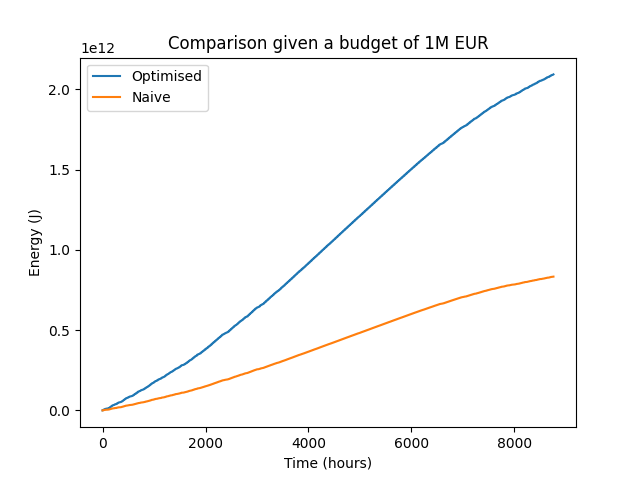
\includegraphics[width=.75\textwidth]{assets/opt_naive_cmp.png}
        \caption{$\mathrm{H_2}$ output over time for optimised and naive budget allocations.}
        \label{fig:opt_naive_cmp}
    \end{subfigure}
    \hfill
    \begin{subfigure}[h]{\textwidth}
        \centering
        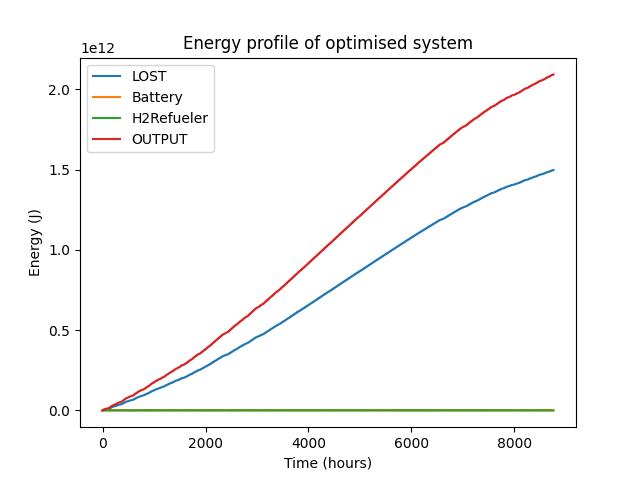
\includegraphics[width=.75\textwidth]{assets/opt_budget_profile.png}
        \caption{Energy distribution through the system over time for optimised budget allocations.}
        \label{fig:opt_budget_profile}
    \end{subfigure}
    \caption{}
    \label{fig:opt_perf}
\end{figure}

\newpage
\section{Conclusion}
A general model was developed and implemented for the purpose of
analysing the behaviour of energy conversion networks.
Using a simple linear system as a demonstration, the model was applied to a techno-economic optimisation problem
with sensible assumptions about component characteristics and yielded sensible results.
\bibliography{refs}


\end{document}